% 编码格式: "TeX:UTF-8"
% tex编译链 = xelatex
% Created by tinoryj on 2017/2/27.
% Copyright © 2017年 tinoryj. All rights reserved.
% 模版支持三级标题,如果需要插入第四级请自行修改cls中217行\setcounter{secnumdepth}{3}中的数值
% lipsum[1] 为模版文字,使用时自行删除
% 基于2011版格式要求设计,针对现行电子版不要求前两页信息进行设计。

\documentclass[bwprint]{cumcmthesis} 
%题目

\title{逢山开路}

\begin{document}
 \maketitle

\begin{abstract}
%变分法

对于给定的地形和必经点的路径规划问题,本文将给出具体的解决方法设计线路使其总造价尽可能低。

本题将需要设计的线路看做一条曲线,将该曲线的切线方向上的方向导数作为约束条件,将造价作为曲线积分的权值,求解得到最优方案。本文将连续曲线简化为离散的线段和进行求解。首先利用双三次插值将数据加细 ,尽可能还原地形来设计更精细的路线。然后我们通过定性与定量分析,分别建立了沿等高线设计路线的方法和动态规划的求解方法。沿等高线设计路线的核心思想是少爬山或下坡让总路线最短从而优化总造价。动态规划模型基于对桥梁和隧道的造价远高于普通公路的考虑。我们需要先优化桥梁和隧道的长度。确定好它们的修建位置后,路线就转化为分段求和问题。而公路路段的造价与长度成正比,通过求解公路的最短路径即可得到最小造价设计方案。我们分别使用Dijkstra算法和SPFA算法求解最短路径然后取最优解。

对于居民点,我们将整个路径划分为山脚到桥、桥、桥到居民点、居民点到隧道、隧道、隧道到矿区共六段路程。因为隧道长度大于300米时价格翻倍,所以将隧道的长度控制在300米之内。通过模型得到一种总长度为10199.65米,造价为357万元的设计方案。
对于居民区,我们保持第一问的设计不变,通过对比分析四个定点确定公路经过居民区的点的坐标为$(3600,2400,1150)$,利用SPFA算法计算得到一种总长度为9392.63米,造价332万元的设计方案。

最后,我们求解了不修建隧道、改变桥梁位置两种情况下的设计方案,造价均在400万元以上,说明我们的方案相对合理且有效。

\keywords{动态规划,\quad 局部最优,\quad 单源最短路径, \quad 坡度}

\end{abstract}

\tableofcontents
\newpage
\section{问题重述}
	我们要在一山区修建公路,已知该山区各点的高程。数据显示:在$y=3200$ 处有一东西走向的山峰;从坐标$(2400,2400)$到$(4800,0)$有一西北——东南走向的山谷;在$(2000,2800)$附近有一山口湖,其最高水位略高于$1350$米,雨季在山谷中形成一溪流。经调查知,雨量最大时溪流水面宽度$w$与(溪流最深处的)$x$ 坐标的关系可近似表示为:
\begin{equation}
	w(x) = (\frac{x-2400}{2})^{3/4}+5\quad (2400 \leqslant x \leqslant 4000)
	\label{河流计算}
\end{equation}

	公路从山脚$(0,800)$处开始,经居民点(4000,2000)至矿区(2000,4000)。已知路段
工程成本及对路段坡度(上升高程与水平距离之比)的限制如表\ref{造价与坡度要求}。
	
\begin{table}[h]
\centering
\caption{造价与坡度要求}
\label{造价与坡度要求}
\begin{tabular}{cccc}
\toprule
工程种类&一般路段&桥梁&隧道\\
\midrule
工程成本(元/米) &300 &2000 & 1500(长度$\leqslant$300米);3000(长度$>$300米)\\
\midrule
对坡度的限制 & <0.125 & =0 & <0.100\\
\bottomrule
\end{tabular}
\end{table}

\begin{enumerate}
	\item 给出一种线路设计方案,包括原理、方法及比较精确的线路位置(含桥梁、隧道),并估算该方案的总成本。
	\item 居民点改为$3600 \leqslant x \leqslant 4000, \quad 2000 \leqslant y \leqslant 2400$的居民区,公路只须经过民区即可,提出修改方案。
\end{enumerate}

概括即:我们需要根据地形(高度)和工程成本来决定一条最佳的线路,本题中我们将总成本作为最终最优化的目标。
	
\section{问题分析}	
在本题中,通过给定的数据表,我们可以得到该山区的地形图,如图(\ref{通过给定数据的到的山区地形图},\ref{河道面地形图})

\begin{figure}[h]  
\begin{minipage}[t]{0.5\textwidth}
\centering  
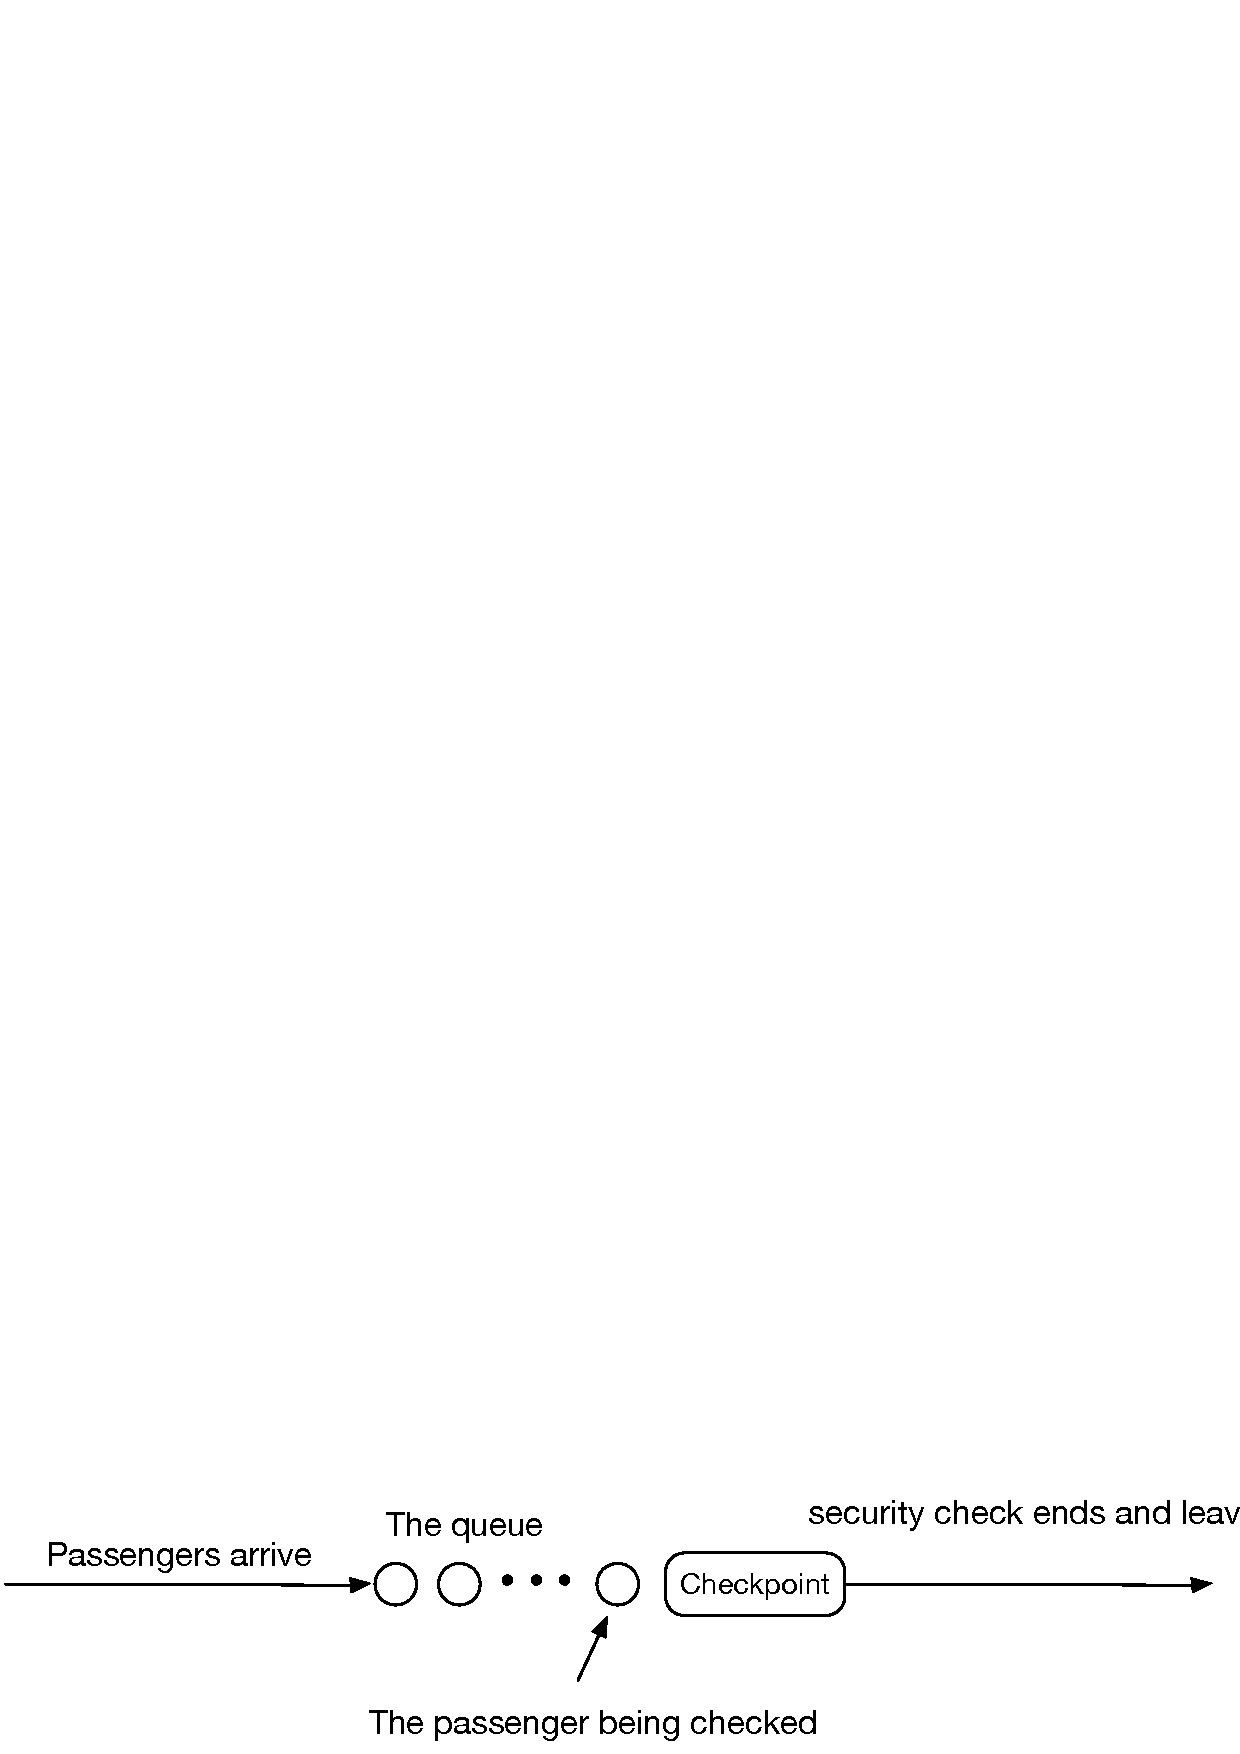
\includegraphics[width=\linewidth]{1.png} \\
\caption{通过给定数据的到的山区地形图} \label{通过给定数据的到的山区地形图}
\end{minipage}
\hspace{1ex}
\begin{minipage}[t]{0.5\textwidth}  
\centering  
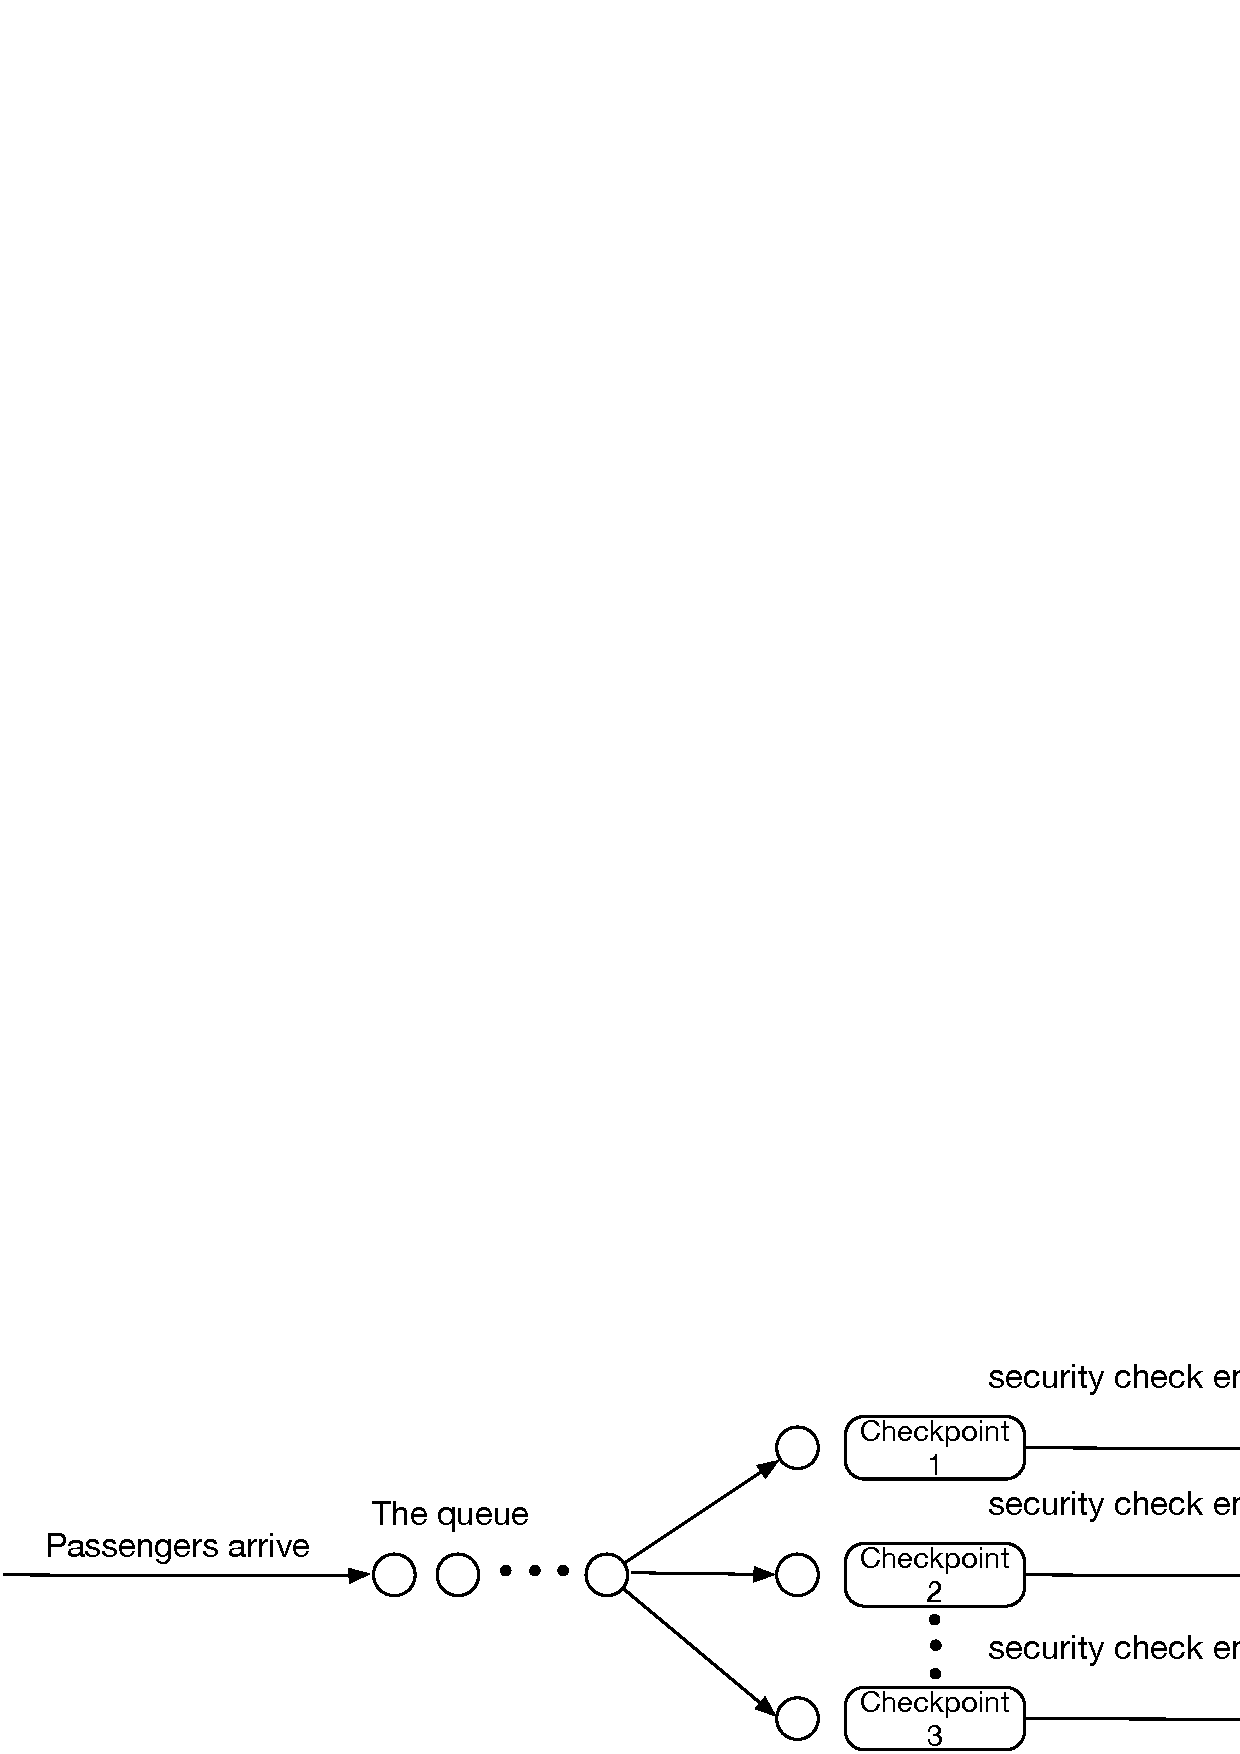
\includegraphics[width=\linewidth]{2.png}\\
\caption{河道面地形图}  \label{河道面地形图}
\end{minipage}  
\end{figure} 

通过观察该地形图,发现直接使用原有数据进行计算难以满足工程中对于不同工程种类的坡度限制要求。同时,采用在格点间修路的方式容易导致出现大角度转弯等现象。我们需要对地形数据进行优化,以满足计算需要。

同时,观察地形图发现在出发点和居民点之间存在一道谷地,在雨季会形成小溪,需要修建桥梁;在居民点和矿区之间存在一高山阻挡,且高山的坡度很大,可能需要考虑修建隧道以缩短盘山公路长度。详见图(\ref{等高线图})。
\begin{figure}[h]
\small
\centering
\includegraphics[width=14cm]{3.png}
\caption{等高线图} 
\label{等高线图}
\end{figure}
 
                                                                                                                                                                                                                                                                        
\section{模型建立}
\subsection{理想模型}
	本题中可将问题一般化抽象为求解最优路线的问题,对于一般给定的路径如图(\ref{示意图})、公式(\ref{len}),可以通过计算该曲线的曲线积分得到路径总长度。同时,为了满足题目条件中的坡度限制要求,分别对不同路段线路的方向导数添加限制条件(\ref{dl}),最终得到路径规划。

\begin{equation}
\label{len}
l : \left\{
\begin{aligned}
x & = & x(t) \\
y & = & y(t) \\
z & = & f(x,y)
\end{aligned}
\right. \quad \quad \quad l = \int_{l}ds
\end{equation}


\begin{equation}
\label{dl}
	\frac{dz}{d\bar{l}} \leqslant K
\end{equation}
其中 K 为不同种类路段的坡度要求。

\begin{figure}[h]
\small
\centering
\includegraphics[width=14cm]{12.png}
\caption{示意图} 
\label{示意图}
\end{figure}

\subsection{求解方案}
针对河流和高山影响,若绕过河流则无法实现目标设定,因此桥梁必须修建。

若考虑修建隧道,则可将全程分为6个部分(起点—桥东侧,桥梁,桥西侧-居民点,居民点-隧道南侧,隧道,隧道北侧-矿区),并且设置4个控制点以分别确定大桥和隧道的修建位置。

若不考虑修建隧道,可将全程分为4个部分(起点—桥东侧,桥梁,桥西侧-居民点,居民点-矿区)。

\subsection{符号声明}
\begin{itemize}
	\item $S$:起点位置$(0,800)$
	\item $B_1$:大桥在峡谷西侧的起始位置(未定)
	\item $B_2$:大桥在峡谷西侧的起始位置(未定)
	\item $P$:居民区$600 \leqslant x \leqslant 4000, 2000 \leqslant y \leqslant 2400$ /居民点$(4000,2000)$
	\item $T_1$:隧道在山峰南侧的起始位置(未定)
	\item $T_2$:隧道在山峰北侧的结束位置
	\item $D$:矿区位置$(2000,4000)$
\end{itemize}

\subsection{基本假设}
\begin{enumerate}
	\item 满足坡度要求,工程上即能够实现修路修隧道或者架桥。
	\item 将地图抽象为离散的点,以简化模型。
	\item 无重大地质灾害。
	\item 路线近似曲线,但相邻细分的点之间均用直线相连。
\end{enumerate}


\section{模型求解前准备}
\subsection{地形数据插值优化}
针对题目给定地形数据量不足,采用双三次插值(立方卷积插值)的方法对原有数据进行加密,使得各个格点间距离减小,便于模型计算时使用。原有数据点间距为400米,我们将其间距插值为50米,将原有每个方格面积缩小为原面积的$\frac{1}{64}$。

双三次插值(立方卷积插值)\upcite{4} 创造的数据点的数值来源于该点附近的$(4\times4)$个数据点,精确度较高。

定义高程数据点集合为F,可以通过公式(\ref{插值公式})得到,
\begin{equation}
	F(i+v,j+u) = ABC
	\label{插值公式}
\end{equation}
其中
$$ A = F(1+u,:)+F(u,:)+F(1-u,:)+F(2-u,:)$$
$$ B = \left[
\begin{matrix}
F(i-1,j-2)&F(i,j-2)&F(i+1,j-2)&F(i+2,j-2)\\
F(i-1,j-1)&F(i,j-1)&F(i+1,j-1)&F(i+2,j-1)\\
F(i-1,j)&F(i,j)&F(i+1,j)&F(i+2,j)\\
F(i-1,j+1)&F(i,j+1)&F(i+1,j+1)&F(i+2,j+1)
\end{matrix}
\right]
$$

$$ C = F(1+v,:)+F(v,:)+F(1-v,:)+F(2-v,:)$$

对数据进行插值计算的具体实现详见附录,经过插值之后,得到了新的山区地形图如图(\ref{插值后得到的山区地形图})所示
\begin{figure}[h]
\small
\centering
\includegraphics[width=14cm]{4.png}
\caption{插值后得到的山区地形图} 
\label{插值后得到的山区地形图}
\end{figure}

\subsection{对河流宽度的计算}
通过对图(\ref{插值后得到的山区地形图})的观察,可以看出:峡谷的谷底基本为直线,峡谷两侧基本对称。
谷底方程可近似为:$x+y = 4800 \quad (2400 \leqslant x \leqslant 4800)$
结合公式(\ref{河流计算})可得:

河岸西侧方程:
\begin{equation}
	4800 - x - y = \frac{\sqrt{2}}{2}\omega \left(\frac{x-y+4800}{2} \right) \quad (2400 \leqslant x \leqslant 4800)
	\label{河岸西侧方程}
\end{equation}

河岸东侧方程:
\begin{equation}
	x + y - 4800 = \frac{\sqrt{2}}{2}\omega \left(\frac{x-y+4800}{2} \right) \quad (2400 \leqslant x \leqslant 4800)
	\label{河岸东侧方程}
\end{equation}

\section{问题一分析与求解}
\subsection{方案一}

通过插值数据得到更为精确的等高线图,为了保证公路的坡度符合要求,沿等高线修建公路,同时为了降低桥梁和隧道的建设成本,通过绕路的方式实现桥梁和隧道长度的最小化。可以得到修建路线图如下图(\ref{公路修建路线图})所示:
\begin{figure}[h]
\small
\centering
\includegraphics[width=14cm]{10.png}
\caption{公路修建路线图} 
\label{公路修建路线图}
\end{figure}

该模型仅可作为粗略的估计方法,沿等高线修路直观、简便、但非常不精确,只能得到大概的路线以及费用估计值。同时,若要在坡度变化较大的地方通过等高线方法修路,必须使用等高线密度足够大的等势图。
由于无法求得具体的路线长度,所以无法估计该修建方法所需的花费。

\subsection{方案二}
本题核心问题为求解从起点S到居民点P再到矿区D两段路经的最短路径,但由于桥梁和隧道的影响,直接求解存在极大困难。因此根据对于地形雨同路段费用系数的分析先确定桥梁和隧道的修建位置\upcite{3}。

在确定大桥和隧道的修建位置之后,剩余四段路均为普通公路。由于桥梁和隧道的建设费用已经确定,若使得工程总费用最小,问题转化为求解四段公路的最短路径。

由于最短路径Dijkstra算法基于二维平面上的带权图,所以需要对插值后的数据进行处理,以便使用最短路径算法求解公路修建路径。

\subsubsection{桥梁位置选择}
通过公式(\ref{河岸西侧方程},\ref{河岸东侧方程})可知,小溪的宽度随x的增加呈递增关系。再从小溪左右公路对坡度要求,我们暂时确定小溪的位置在点之间,因为小溪的直线方程从点开始为:
$$ P_{start}=\left\{
\begin{aligned}
x & = & 2800+400t \\
y & = & 2000-400t \\
z & = & 900-200t
\end{aligned}
\right.
$$

通过计算发现,在小溪上游与下游修建桥梁的长度差距在50米以内,但在最上游修建桥梁虽然可以使得桥长最短,但会导致第一段普通公路严重绕行,在下游修桥更会导致桥长和第一段公路长度的大大加长,因此我们先假设在小溪中心高程$z=800$的地方修桥。在这样的高程上,我们找到小溪上对应的点为$B(3000,1800,800)$,由此算出溪流的宽度:$\omega(3000)=77.084M$。

由于桥梁的建设要求坡度为零,从这方面考虑,则桥的两个落点只能在点$B_{11}$
$(2800,1600,1300)$,
$B_{21}(3200,2000,1100)$这两点与A点的两条直线上确定,为了使得桥的宽度最接近于小溪宽度,通过计算,我们求得桥的两端点为$B_{1}(2978,1788,855)$,
$B_{2}(3036,1836,855)$,则桥的实际高程为855米,桥的实际宽度为82米。桥梁修建位置如下图(\ref{桥梁修建位置})所示。

\subsubsection{隧道位置选择}
由题目所给数据容易看出,修建隧道的成本很高,特别是当隧道长度超过300米时,成本会激增1倍,达到普通公路修建成本的10倍,因此我们应当尽量选取宽度在300米以内的山峰处修建隧道,通过等高图(\ref{等高线图})可以发现在$x=4400M$处的山峰非常尖锐,非常适合于修建隧道以节约成本,因此在以下的计算中,我们固定隧道的x坐标为$x=4400M$。

为了使得隧道长度小于300米,我们需要通过修建盘山公路的方式将公路高度抬升到一定高度,对于水平隧道
$$Z_c = 1500-\frac{300\times650}{400\times(1+\frac{650}{600})} = 1266$$
由于隧道的坡度限制条件为$\alpha \leqslant 0.100$通过数据表可知矿区海拔高度为1320米,考虑修建一条南高北低的隧道,同时令隧道坡度小于临界值0.100,通过计算得到了隧道南北两侧的定位点$T_1(4400,3050,1341)$,$T_2(4400,3350,1329)$
修建的隧道位置如图(\ref{隧道修建位置})所示。

\begin{figure}[h]  
\begin{minipage}[t]{0.5\textwidth}
\centering  
\includegraphics[width=\linewidth]{6.png} \\
\caption{桥梁修建位置} \label{桥梁修建位置}
\end{minipage}
\hspace{1ex}
\begin{minipage}[t]{0.5\textwidth}  
\centering  
\includegraphics[width=\linewidth]{5.png}\\
\caption{隧道修建位置}  \label{隧道修建位置}
\end{minipage}  
\end{figure} 

\subsubsection{普通公路修建位置选择-Dijkstra算法}
对于普通公路,我们采用适用于稠密图且复杂度仅为$o(nlogn)$的Dijkstra最短路径算法进行求解。该算法的核心思想是以起始点为中心向外层层扩展,直到扩展到终点为止。

\textbf{动态规划Dijkstra算法的设计思路}

\begin{enumerate}
	\item 首先,引入一个辅助向量$D$,它的每个分量$D[i]$表示当前所找到的从起始点$v$(即源点$v$)到其它每个顶点$v_i$的长度。
	\item D的初始状态为:若从$v$到$v_i$有弧(即从$v$到$v_i$存在连接边),则$D[i]$为弧上的权值(即为从$v$到$v_i$的边的权值);否则置$D[i]$为$\infty$。

		显然,长度为$D[j]= Min{ D |v_i \in V}$的路径就是从$v$出发到顶点$v_j$的长度最短的一条路径,此路径为$(v,v_j)$。
	\item 找到对于下一条长度次短的一条边,也就是找到从源点$v$到下一个顶点的最短路径长度所对应的顶点,且这条最短路径长度仅次于从源点$v$到顶点$v_j$的最短路径长度。
 
	假设该次短路径的终点是$v_k$,则可想而知,这条路径要么是$(v,v_k)$,或者是$(v,v_j,v_k)$。它的长度或者是从$v$到$v_k$的弧上的权值,或者是$D[j]$加上从$v_j$到$v_k$的弧上的权值。
	\item 一般情况下,假设$S$为已求得的从源点$v$出发的最短路径长度的顶点的集合,则可证明:下一条次最短路径(设其终点为$x$)要么是弧$(v,x)$,或者是从源点$v$出发的中间只经过$S$中的顶点而最后到达顶点$x$的路径。

	因此,下一条长度次短的的最短路径长度必是$D[j]= Min { D[i] |v_i \in V-S}$,其中$D[i]$要么是弧$(v,v_i)$上的权值,或者是$D[k](v_k \in S)$和弧$(v_k,v_i)$上的权值之和。
\end{enumerate}

\textbf{针对本问题的处理}

在本问题中,我们拥有的并不是二维平面上的带权值图,而是三维空间上的高程图,因此我们需要通过一种算法将三维空间中的高度信息转化为二维图中的边权值信息。

考虑到普通公路修建是需要满足坡度条件:$\alpha \leqslant 0.125$,我们考虑在将高程信息表中网格通过双三次插值的方法将网格从$400\times 400$加密到$10\times 10$,以便于每个顶点找到前往附近8各顶点的通路。

将插值之后的每个格点视作二维平面图的顶点,我们针对每个顶点邻接的8顶点计算其权值。邻接方式如下矩阵所示:

$$\left[
\begin{matrix}
P(i-1,j-1)&P(i-1,j)&P(i-1,j+1)\\
P(i,j-1)&P(i,j)&P(i,j+1)\\
P(i+1,j-1)&P(i+1,j)&P(i+1,j+1)
\end{matrix}
\right]
$$

考虑到普通公路的坡度限制之后,我们将两顶点间边的坡度大于0.125的边看作非通路($\infty$),通过如下公式()对每个顶点的边权值进行计算,具体实现详见附录。

\begin{equation}
d_{ij}=\left\{
\begin{array}{lr} 
[(\Delta x)^2+(\Delta y)^2+(\Delta z)^2]^{1/2} & \frac{|\Delta z|}{[(\Delta x)^2+(\Delta z)^2]^{1/2}} \leqslant 0.125\\
\infty & \frac{|\Delta z|}{[(\Delta x)^2+(\Delta z)^2]^{1/2}} >0.125
\end{array}
\right.
\end{equation}

\subsubsection{结果与分析}

通过计算,得到工程设计方案如下图(\ref{结果路线图})所示,工程费用如表(\ref{工程费用表一})所示。

\begin{figure}[h]
\small
\centering
\includegraphics[width=14cm]{7.png}
\caption{结果路线图} 
\label{结果路线图}
\end{figure}

\begin{table}[h]
\centering
\caption{工程费用表一}
\label{工程费用表一}
\begin{tabular}{|c|c|c|c|c|c|c|c|}
\hline
 项目 & 桥梁 & 隧道 & 普通公路 & 总计\\ \hline
长度    & 82米   & 304.3米  & 9813.35米 & 10199.65米 \\ \hline
造价    & 164000元 & 462900元 & 2944005元 &3570905元\\
\hline
\end{tabular}
\end{table}


\section{问题二模型与求解}
\subsection{方案一}
与第一问中的情况相似,沿等高线修路的方法只能得到粗略的线路方向,如下图(\ref{公路修建线路图2})所示:
\begin{figure}[h]
\small
\centering
\includegraphics[width=14cm]{11.png}
\caption{公路修建线路图} 
\label{公路修建线路图2}
\end{figure}


\subsection{方案二}
对于第二问,题目条件仅仅改变了居民点的范围,因此只需要针对第一问模型中从桥梁东岸到居民点和从居民点到隧道南侧入口的两段普通公路进行修改即可。
\subsubsection{动态规划SPFA算法}
考虑到分段之后,每一段路可以抽象为单源路径,故考虑采用单源最短路算法SPFA对第二问进行求解,其在Bellman-ford算法的基础上加入队列优化,减少了冗余的松弛操作,极大提高了算法效率。有助于更快的求解出所需的结果。

\textbf{算法设计思路}

通过建立一个队列,初始时队列里只有起始点,再建立一个表格记录起始点到所有点的最短路径(该表格的初始值要赋为极大值,该点到他本身的路径赋为0)。然后执行松弛操作,用队列里有的点作为起始点去刷新到所有点的最短路,如果刷新成功且被刷新点不在队列中则把该点加入到队列最后。重复执行直到队列为空。最终得到最短路径所经过的各个顶点的列表。

沿用第一问中对于数据的处理以及获得的地形图各顶点的邻接矩阵进行计算。

\subsubsection{分段点的确定}

通过图(\ref{居民区位置})可以发现,若使得普通公路尽量减少绕行,应当从居民区左上角一点处通过,其余各个分段点与第一问保持不变。

\begin{figure}[h]
\small
\centering
\includegraphics[width=14cm]{8.png}
\caption{居民区位置} 
\label{居民区位置}
\end{figure}

\subsubsection{结果与分析}
通过SPFA算法分段计算最短路径,得到工程设计方案如下图(\ref{结果路线图2})所示,工程费用如表(\ref{工程费用表二})所示。

\begin{figure}[h]
\small
\centering
\includegraphics[width=14cm]{9.png}
\caption{结果路线图} 
\label{结果路线图2}
\end{figure}

\begin{table}[h]
\centering
\caption{工程费用表二}
\label{工程费用表二}
\begin{tabular}{|c|c|c|c|c|c|c|c|}
\hline
 项目 & 桥梁 & 隧道 & 普通公路 & 总计\\ \hline
长度    & 82米   & 304.3米  & 9006.33米 & 9392.63米 \\ \hline
造价    & 164000元 & 462900元 & 2701899元 &3328799元\\
\hline
\end{tabular}
\end{table}

\section{方案合理性分析}
由于求解所有可能情况存在计算上的极大困难,因此我们优先采用了固定桥梁隧道位置的方法对方案与求解进行简化,但这种简化使得我们的方案只能确保为可行方案,但无法保证方案对成本足够节约。因此我们通过分析改变桥梁位置、采取修建盘山路来避免修建隧道这两种不同方案,来验证我们方案的成本是否相对较优。

对于需要验证的两种方案,在求解时除确定桥梁隧道位置外,均采用最短路径的方法进行求解。

\subsection{不修建隧道}
\begin{figure}[h]  
\begin{minipage}[t]{0.5\textwidth}
\centering  
\includegraphics[width=\linewidth]{13.png} \\
\caption{居民点} \label{居民点2}
\end{minipage}
\hspace{1ex}
\begin{minipage}[t]{0.5\textwidth}  
\centering  
\includegraphics[width=\linewidth]{14.png}\\
\caption{居民区}  \label{居民区2}
\end{minipage}  
\end{figure} 

\begin{table}[h]
\centering
\caption{不修建隧道时工程总费用}
\label{不修建隧道时工程总费用}
\begin{tabular}{ll}
\toprule
方案 & 费用\\
\midrule
方案一:居民点,不修建隧道 & 4126064元\\
方案二:居民区(过点$(3600,2000)$),不修建隧道 & 3679765元\\
\bottomrule
\end{tabular}
\end{table}

\subsection{改变桥梁位置}
修改桥梁位置到点$B_1(3200,1200)$,$B_2(3200.1600)$之间,桥长为110.737米。计算发现居民点变为居民区对于该种桥梁修建方案无影响。
进而修改隧道修建位置到$x = 4600$处,隧道长度可缩短为280.00米。计算所得路线规划如下图(\ref{方案路线图})所示,总造价为4626928元。调整为居民区后路径与造价不变。 

\begin{figure}[h]
\small
\centering
\includegraphics[width=13cm]{15.png}
\caption{方案路线图} 
\label{方案路线图}
\end{figure}

通过对两种情况的分析,可以看出,我们的方案相对于不修隧道、修长桥短隧道的方案更优。可以基本保证方案相对较优。

\section{模型评价与改进方向}
\subsection{模型的评价}
\subsubsection{优点}
\begin{enumerate}
	\item 通过双三次插值的方式,尽可能精确的获得了计算所需的必要数据。
	\item 对于模型一,简单直观,便于直接观察设计修建方案。
	\item 对于模型二,Dijkstra算法与SPFA算法的应用,通过动态规划的方式实现各段公路的最优化求解。
\end{enumerate}
\subsubsection{不足}
\begin{enumerate}
	\item 对于模型一,无法精确的进行计算,只能简单观察和设计路径,使用价值一般。
	\item 对于模型二,主观定义桥梁和隧道的修建位置使得整体的解无法保证最优。
	\item 在模型二中,使用最短路径算法存在计算困难的问题,因此细分网格点只能精确到$(100\times100)$米的网格进行计算,结果不够精确。且在部分转弯处出现超大角度转弯,不符合实际。
\end{enumerate}
\subsection{模型的改进方向}
\begin{enumerate}
	\item 将桥梁位置、隧道位置、居民区边界选点全部纳入动态规划的范围之内,避免主观确定位置带来的影响。
	\item 改进最短路径算法,换用C++实现,提高计算效率,避免过长时间的计算。
	\item 先通过原有网格点进行动态规划搜索,实现较低复杂度下的全局动态规划。确定控制点之后在相邻控制点间继续细分搜索区域,避免了数据量过大导致的计算不可能问题,又增加了模型精确度。

\end{enumerate}






\begin{thebibliography}{9}
 \bibitem{3} 孙长银, 杨峤, 黄琼. 逢山开路的数学模型[J]. 三峡大学学报(人文社会科学版), 1998(1):25-28.
 \bibitem{4} 冯仁忠, 查理. 局部构造$C^2$连续的三次B样条插值曲线和双三次插值曲面[J]. 图学学报, 2005, 26(6):110-117.
 
 \bibitem{1} \url{https://en.wikipedia.org/wiki/Shortest_Path_Faster_Algorithm}
 \bibitem{2} \url{https://en.wikipedia.org/wiki/Dijkstra}

\end{thebibliography}

\section{附录:相关程序}
\subsection{地型相关图形绘制}
\lstinputlisting[language=Matlab]{./code/dar.m}
\subsection{地形图抽象化为邻接矩阵}
\lstinputlisting[language=Matlab]{./code/calu.m}
\subsection{Dijkstra算法实现}
\lstinputlisting[language=Matlab]{./code/dijk.m}
\subsection{SPFA算法实现}
\lstinputlisting[language=C++]{./code/spfa.cpp}


\end{document} 